\documentclass[11pt, a4paper]{article}

\usepackage[utf8]{inputenc}
\usepackage[italian, english]{babel}
\usepackage[pages=some]{background}
\usepackage{hyperref}
\usepackage{float}
\usepackage{amsmath}

\graphicspath{ {./img/} }
\backgroundsetup{
	firstpage = {true},
	placement = {center},
	position = current page.center,
	contents = {
\includegraphics[scale=0.07]{unipd}},
	angle = {0},
	opacity = {0.03}
}
\hypersetup{
	colorlinks=true,      
	urlcolor=blue,
	linkcolor=black
}

\newcommand{\image}[3]{
	\begin{figure}%[H]
		\centering
		\includegraphics[width=0.9\textwidth]{#1}
		\caption{#2.}
		\label{#3}
	\end{figure}
}

\title{Vision and Cognitive Services\\
\large Video Frame Interpolation via Adaptive Separable Convolution}
\author{Filippo Visentin (matricola)\\
Nicola Carlesso (1237782)}
\date{a.a. 2020/2021}

\begin{document}
	\maketitle
	\newpage
	
	\tableofcontents
	\newpage
	
	\section{Introduction}
	Our work is related on the video frame interpolation problem. In particular we look at work in \cite{mainpaper}.\\
	The video frame interpolation problem consists of recreating the frame between two input frames in a video. This problem allows either to obtain a higher quality video, in terms of frames per second, or a more defined slow motion, or a super slow motion.\\
	The main challenge of this problem is to get an output frame with defined images, because the network tends to give in output a blurred frame, and recreate a good frame in case of two input frames are quite different.\\
	Our network has a decoder-encoder architecture, used mainly to recreate fake example from a dataset, as in our case study. The network doesn't create directly the interpolated frame, but gives in output an ad hoc couple of kernels for each input frame. As last step we apply the convolutional operation with output kernels and input frames to get the output frame. 
	
	\section{Related work}
	Other approaches to resolve this problem are with the optical flow technique \cite{optical_flow}, where the network learns the movements of figures in the frame and predicts those immediately following. This technique requires two steps: first estimate optical flow between input frames and then synthesize an intermediate frame guided by motion; our approach has instead a single convolution process.\\
	The work we rely on is a continuation of another work in \cite{previous_work} that use our same network structure with one, mainly difference: in our network we obtain two kernels for each input frame, a column vector and a row vector, in \cite{optical_flow} the network gives one standard kernel (a square matrix) for each input frame. The first improvement with the network of \cite{mainpaper} is the memory and the time, because the network gives only a column and a row vector, instead of a matrix, in fact the usage of memory went from 26GB and 1.27GB.  In this way,	an $n\times n$ convolution kernel can be encoded using only $2n$ variables.\\
	Another improvement is the sharpness and quality of output frames.
	
	\section{Dataset}
	Fortunately, for the video frame interpolation problem its easy to create a large dataset, without looking online.\\
	We just have to take a video and extract a triplet of close frames. The input are the first and last frame of triplet, and the label is the second frame. Its important consider two factors:
	\begin{itemize}
		\item all frames in triplet must be enough different, otherwise the example will be useless for the learning phase;
		\item all frames in triplet don't must be too much different. For example, in the case of in the middle of triplet a change of scene occurs. 
	\end{itemize}
	Therefore, we have setted a lower and an upper bound for the difference between frames in the triplet.\\
	The magnitude of motion is estimated by computing the histogram of the 2 frames, and comparing them by taking the norm of the difference vector. \\
	Another important hyper-parameter used to create the database is the number of frames between elements of the triplet. In this way we have examples that can show more os less movement, so we can test strength of the network.\\
	To create our dataset we use \href{https://www.crcv.ucf.edu/data/UCF101.php}{UCF-101} and the Python script\\ \texttt{dataset/create\_dataset-py}. We use a dataset with about 6000 examples.
	%% iniziare avendo scritto circa 2 pagine
	\section{Method} %% quasi 2 pagine
	The structure of the CNN used is based on that of \cite{mainpaper}, showed in Figure~\ref{original-net}, with some changes. At the core there is a sequence of encoding convolutional layers, separated by pooling layers, followed by a sequence of decoding layers with upscaling (bilinear). The upscaling reintroduces feature maps from the encoding layer, in order to facilitate the decoding. As output of the net we expect a couple of separable kernels for each pixel, used to combine pixels from the 2 input frames to obtain each new pixel of the interpolated frame. \\
	In the network use used the skip connection technique to let the expanding	layers incorporate features from the contracting part of the neural network.\\
	If we call $I_1$ and $I_2$ two input frames and $\hat{I}$ the interpolated frame, to compute each output pixel $(x,y)$, the final stage applies at each input frame a convolutional operation between every output kernel and patches centred in $(x,y)$.\\
	As we ca see in Figure~\ref{original-net}, if we consider inputs like a matrix $128\times128$ and we set the size of separable kernels as $51\times1$, the output of network are four matrices $51\times128\times128$: $k_{1,h}$, $k_{1,v}$, $k_{2,h}$, $k_{2,v}$. We consider $k_{n,s}(x,y)$ as a vector $51\times1$, and we call $K_n(x,y) = k_{n,h}(x,y) * k_{n,v}(x,y)$, a matrix $51\times51$, and the input patch centred in $(x,y)$ of frame \textit{n} $P_n(x,y)$, always a matrix $51\times51$.
	
	\begin{equation}
		\hat{I}(x,y) = Conv(K_1(x,y), P_1(x,y)) + Conv(K_2(x,y), P_2(x,y))
	\end{equation}
	
	\image{net_structure}{Structure of original convolutional network}{original-net}

	\section{Experiment} %% quasi 2 pagine
	In order to improve the performance of the network we explored many solutions, some of which not useful and some more interesting.\\
	We added \textbf{normalization} to the input images with successive denormalization on output images, by calculating mean and variance, in order to obtain a better learning. That has proven ineffective, as images were already nearly normalized by their own. \\
	We tried \textbf{dropout}, but without any noticeable difference in accuracy.\\
	We tried to change \textbf{optimizer} but the best remains Adam.\\
	An interesting improvement we introduced, is to simply remove a convolutional layer every 4, leaving the other 3. This way the time per epoch reduces by about 30\% and the network trains faster without the risk of under fitting. In fact the network is able to overfit (if given enough epochs) even large datasets.
	
	\subsection{Loss function}
	The original loss is a simple \textbf{Mean Squared Error} between pixels of the predicted image and the real one. \\
	To improve on that we tried to compare the feature maps given as output of one of the intermediate layers of the \textbf{VGG-19} net. This is because a one one comparison of pixels focuses on really fine details and looses on the overall (local) appearance of the image. VGG-19 extracts features, focusing more on discriminative information (for classification) than e.g. noise. \\
	We found that taking an early layer of the VGG-19 net given a more interesting loss: at late layers the loss focuses on overall shapes, this way our net tries harder to match the shape instead of its position on the image. 
	\image{mse_loss2}{The Mean square error loss is blurry}{loss-mse}
	\image{vgg16_relu4_4_loss2}{Taking the VGG-19 at a late layer makes our network choose between one of the 2 inputs}{loss-vgg19-44}
	\image{vgg16_relu2_1_loss2}{Taking it at a early layer gives some sort of trade off}{loss-vgg19-21}
	
	Following the idea of using feature maps to create a loss function, we decided to try some handcrafted filters.
	\begin{figure}
		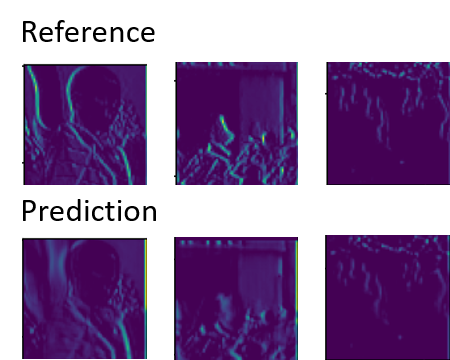
\includegraphics[width=.5\textwidth]{map_sobel}
		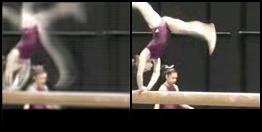
\includegraphics[width=.3\textheight]{sobel}
		\caption{Using a \textbf{sobel} filter we try to focus on edges, so output images remain defined. Here we show also the feature maps obtained}
		\label{feature-map}
	\end{figure}
	\begin{figure}
		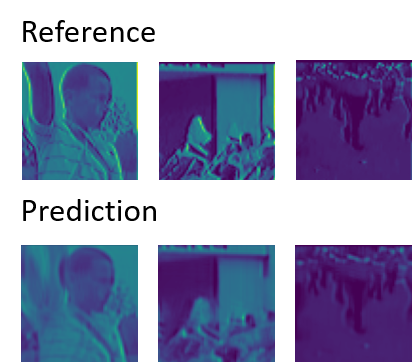
\includegraphics[width=0.3\textheight]{sobel_color_map}
		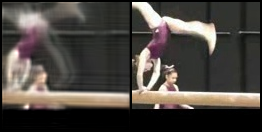
\includegraphics[width=0.3\textheight]{sobel_color}
		\caption{To avoid losing all the information on color, we modified the filter to also consider a bit the central pixel \textbf{color}}
		\label{color-feature-map}
	\end{figure}
	We decided to use the last one at the end as the use of VGG-19 makes the learning slower and also because it retains color information without loosing too much on definiteness.

	\subsection{Image refining layers}
	\subsection{Dvd Logo}
	
	\section{Conclusion}
	
	\bibliographystyle{unsrt}
	\bibliography{bibliography}
	
\end{document}